\section{End-to-End Generation with Empirical \texorpdfstring{$Z$}{Z} Sampling}
\label{app:empirical-unit-cell-z}

The main structure-generation experiments in \Cref{sec:benchmarks} assume known formula-unit count $Z$ for comparison with CLARI. Here, we evaluate an end-to-end setting in which $Z$ is unknown and sampled from an empirical prior estimated from the training set.

\textbf{Prior construction.}
For each training crystal, we group identical molecular components by exact
component SMILES. Let $n_k$ denote the number of copies of distinct component
$G_k$ in the unit cell. We recover the formula-unit count $Z$ and reduced
stoichiometry $\mathbf r$ as
\begin{equation*}
Z=\gcd(n_1,\ldots,n_K),
\qquad
r_k=\frac{n_k}{Z}.
\end{equation*}
We apply this procedure to all 912{,}807 structures in the CLARI training split
after the 512-atom filter. If $c_z$ denotes the number of structures with
$Z=z$, the empirical prior is
\begin{equation*}
\widehat p_{\mathrm{train}}(Z=z)
=\frac{c_z}{\sum_{z'}c_{z'}}.
\end{equation*}
The resulting support is
$\{1,2,3,4,5,6,7,8,9,10,12,14,15,16,18,20,24,26,27,28,30,32,34,40\}$.

\textbf{Sampling formula-unit count $Z$.}
Let $N_{\mathrm{fu}}=\sum_k r_kN_k$ denote the number of atoms in one formula
unit for a benchmark target. To bound inference cost, we restrict $Z$ to values
that yield at most $N_{\max}=4096$ atoms and renormalize the empirical prior:
\begin{equation*}
\widehat p_{\mathrm{trunc}}(Z=z)
=
\frac{\widehat p_{\mathrm{train}}(Z=z)
\,\mathbf{1}[N_{\mathrm{fu}}z\leq N_{\max}]}
{\sum_{z'}\widehat p_{\mathrm{train}}(Z=z')
\,\mathbf{1}[N_{\mathrm{fu}}z'\leq N_{\max}]}.
\end{equation*}
For each candidate, we sample $Z$ from $\widehat p_{\mathrm{trunc}}$, replicate the formula unit accordingly, and pass the resulting unit-cell composition to \model{}. All other settings match the main benchmark.

\textbf{Results.}
We evaluate \model{}-M and \model{}-L with empirical $Z$ sampling and find that
both remain competitive in this end-to-end setting.
\Cref{fig:empirical-z-benchmark,fig:empirical-z-benchmark-exact,fig:empirical-z-benchmark-strict,fig:empirical-z-benchmark-exact-strict}
compare empirical-$Z$ sampling with the main supplied-$Z$ setting at effective
30-candidate and exact 1{,}000-candidate budgets under both standard and strict
criteria. \Cref{fig:empirical-z-candidate-budget} shows how the
supplied and empirical performance gap changes with candidate budget on the Rigid and Flexible benchmarks.

\begin{figure}[H]
  \centering
  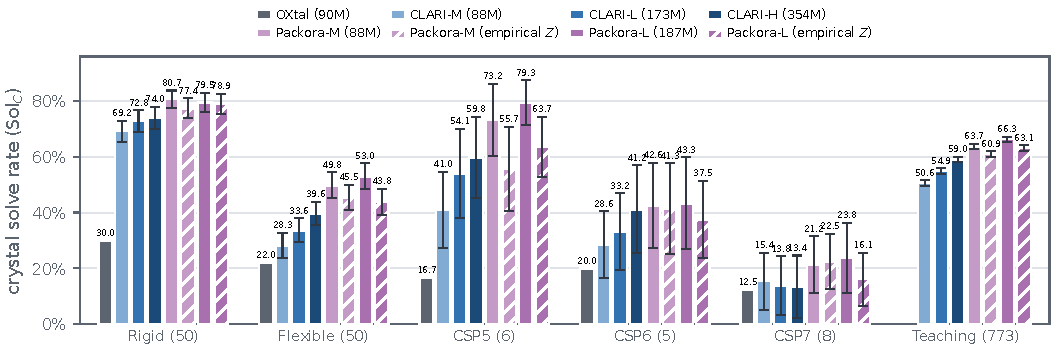
\includegraphics[width=\textwidth]{figures/generated/fig_empirical_z_benchmark.pdf}
  \caption{\textbf{Crystal coverage with empirical unit-cell $Z$ sampling at 30 candidates per target.}
  The solid bars reproduce \Cref{fig:benchmark-teaser}; diagonally hatched bars
  represent results with $Z$ sampled from an empirical prior. Bars report mean
  $\mathrm{Sol}_C$, and error bars show one standard deviation across 5{,}000
  resamples with replacement from each 1{,}000-candidate pool.}
  \label{fig:empirical-z-benchmark}
\end{figure}

\begin{figure}[H]
  \centering
  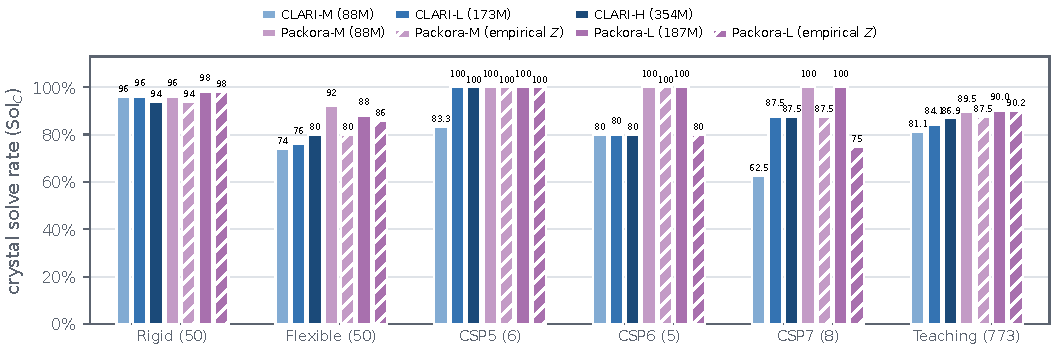
\includegraphics[width=\textwidth]{figures/generated/fig_empirical_z_benchmark_exact.pdf}
  \caption{\textbf{Crystal coverage with empirical unit-cell $Z$ sampling at
  1{,}000 candidates per target.}
  The solid bars reproduce \Cref{fig:benchmark-exact}; diagonally hatched bars
  represent results with $Z$ sampled from an empirical prior. Bars report exact
  $\mathrm{Sol}_C$ over the full 1{,}000-candidate pools.}
  \label{fig:empirical-z-benchmark-exact}
\end{figure}

\begin{figure}[H]
  \centering
  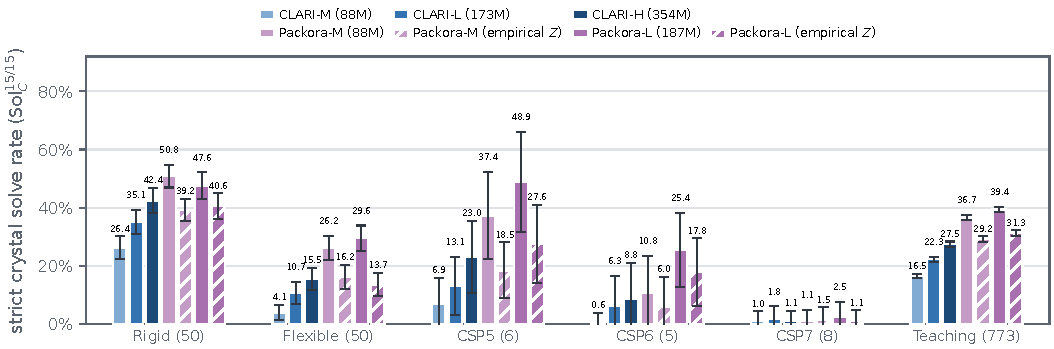
\includegraphics[width=\textwidth]{figures/generated/fig_empirical_z_benchmark_strict.pdf}
  \caption{\textbf{Strict crystal coverage with empirical unit-cell $Z$ sampling
  at 30 candidates per target.}
  The solid bars reproduce \Cref{fig:benchmark-teaser-strict}; diagonally hatched
  bars represent results with $Z$ sampled from an empirical prior. Bars report
  mean $\mathrm{Sol}_C^{15/15}$, and error bars show one standard deviation
  across 5{,}000 resamples with replacement from each 1{,}000-candidate pool.}
  \label{fig:empirical-z-benchmark-strict}
\end{figure}

\begin{figure}[H]
  \centering
  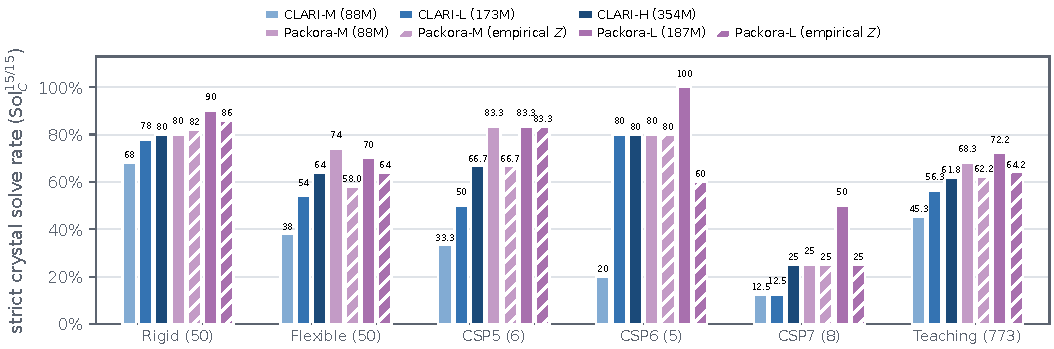
\includegraphics[width=\textwidth]{figures/generated/fig_empirical_z_benchmark_exact_strict.pdf}
  \caption{\textbf{Strict crystal coverage with empirical unit-cell $Z$ sampling
  at 1{,}000 candidates per target.}
  The solid bars reproduce \Cref{fig:benchmark-exact-strict}; diagonally hatched
  bars represent results with $Z$ sampled from an empirical prior. Bars report
  exact $\mathrm{Sol}_C^{15/15}$ over the full 1{,}000-candidate pools.}
  \label{fig:empirical-z-benchmark-exact-strict}
\end{figure}

\begin{figure}[H]
  \centering
  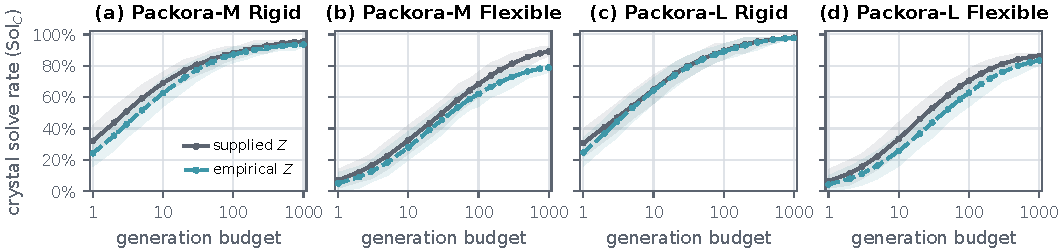
\includegraphics[width=\textwidth]{figures/generated/fig_empirical_z_candidate_budget.pdf}
  \caption{\textbf{Effect of empirical unit-cell $Z$ sampling across candidate budgets.}
  Curves show mean $\mathrm{Sol}_C$ for \model{}-M and \model{}-L on the Rigid
  and Flexible benchmarks over 5{,}000 resamples, and shaded bands show the
  2.5th--97.5th percentiles. The gray solid lines denote supplied $Z$, and the
  teal dotted lines denote empirical $Z$. The two settings remain close across
  candidate budgets.}
  \label{fig:empirical-z-candidate-budget}
\end{figure}
